The aim of this project is to simulate the behavior of voltages and currents in a lossless transmission line in function of time and space. To accomplish this objective, the Finite-Difference Time-Domain method (FDTD) was used. This method makes use of a leapfrog scheme in both time and space and turns a continuous problem in discrete equations. The transmission line studied in this project is depicted in Figure~\ref{fig:TL} and its discretized version in Figure~\ref{fig:TLD}.

\begin{figure}[h!]
    \centering
    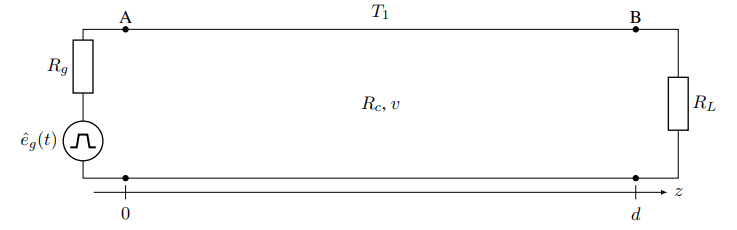
\includegraphics[scale=0.75]{figures/TL.png}
    \caption{Transmission line}
    \label{fig:TL}
\end{figure}

\begin{figure}[h!]
    \centering
    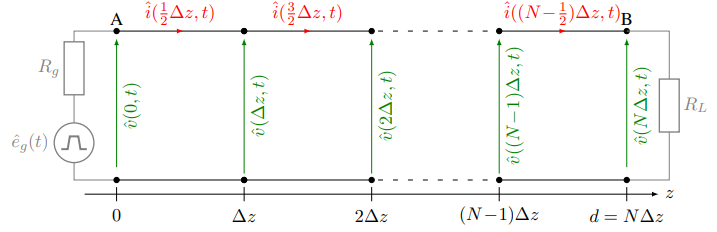
\includegraphics[scale=0.75]{figures/TLD.png}
    \caption{Discretization of the transmission line}
    \label{fig:TLD}
\end{figure}

In the first section, the correct update equations and constants are derived. Using this information, the behavior of a bit traveling through the transmission line is studied, both with default values and with varying parameters. This is all considered with just a resistor as load. Eventually a capacitor is added in parallel to the load. This changes the bit behavior substantially. To conclude the report, an application of transmission line theory inside the field of biomedical engineering is discussed.